\section{实验装置的创新应用}


本项目训练的单摆目标检测模型具有精准度高、性能好的特点,可以广泛应用于物理实验教学中,有效简化实验数据测量步骤,显著提高测量精准度,并实现实验装置的轻量化。通本团队自主开发的实验教学软件,结合训练好的模型进行单摆运动的实时识别,输出单摆的运动时间与坐标信息,实现了AI技术与物理实验的深度融合,为物理实验的观察与数据测量提供了\textbf{智能化辅助}。

\subsection{重力加速度测量的教学创新应用}

单摆运动是中学生接触到的第一个周期性运动,在中学物理教学中设计了通过单摆测量重力加速度的经典实验。然而,传统实验方法存在以下明显不足:

\begin{enumerate}[leftmargin=*]
    \item 人工计时误差大:依赖学生使用秒表手动计时,反应延迟和操作不当导致误差累积;
    
    \item 实验成功率低:为减小随机误差,通常需要测量50个周期左右的总时间并取平均值,过程繁琐且易出错;
    
    \item 摆角限制严格:必须保证单摆在小角度(通常<5°)范围内摆动,否则简谐近似失效,导致系统性误差。
\end{enumerate}

针对这些问题,目前教学中尝试使用的改进方案及其局限性如下:

\begin{itemize}
    \item 光电门计时法:虽然提高了计时精度,但设备成本高、体积大、安装调试复杂;
    
    \item 气垫导轨法:解决了摩擦问题,但装置笨重、价格昂贵,基层学校难以普及;
    
    \item 平衡法与复摆法:理论上可提高准确度,但操作流程复杂,不易为初学者掌握。
\end{itemize}

\begin{figure}[H]
    \centering
    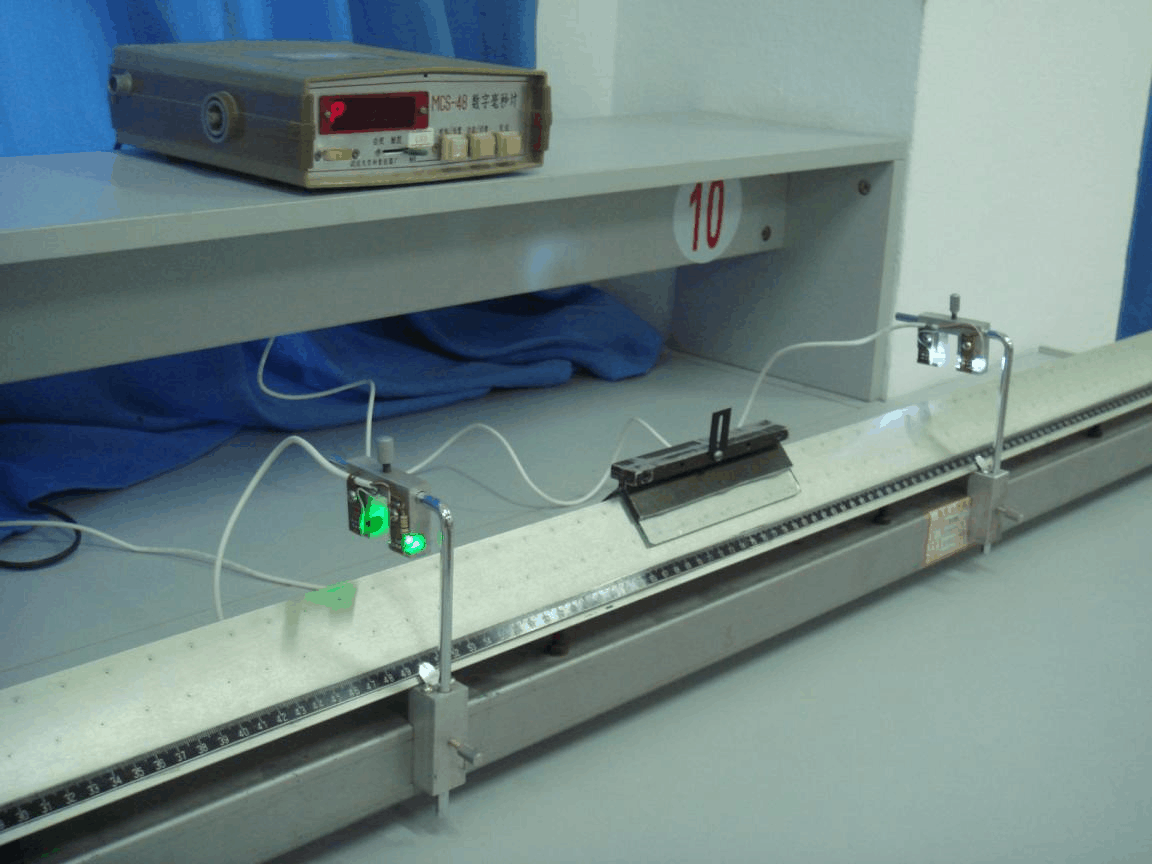
\includegraphics[width=0.6\textwidth]{figures/气垫导轨.png}
    \caption{气垫导轨装置}
    \label{fig:air_track}
\end{figure}

相比之下,本项目提出的基于YOLO AI视觉模型的测量方案具有显著优势:

\begin{enumerate}[leftmargin=*]
    \item 高精度数字化测量:模型可实时追踪摆球位置,精确记录完整运动轨迹,自动计算周期,消除人工计时误差;
    
    \item 低成本简易实现:仅需普通单摆装置和教学电脑即可完成,无需额外专业设备;
    
    \item 操作便捷友好:软件界面直观,学生只需拍摄视频并导入系统,即可获取完整数据集与分析结果;
    
    \item 物理原理可视化:系统自动生成位置-时间曲线,直观展示简谐运动特性,增强学生的物理概念理解。
    
\end{enumerate}

\subsection{阻尼系数测量的的教学创新应用}

在大学物理教学中,阻尼振动是重要的实验内容,但传统教学中学生对振动的位移-时间关系以及速度-时间关系缺乏感性认识。常见的沙摆留迹演示法存在如下明显缺陷:

\begin{enumerate}[leftmargin=*]
    \item 重心位置变化:随着沙的流出,沙漏的重心下降,导致单摆的摆长逐渐变长,周期随之变长,干扰了阻尼效应的观察;
    
    \item 匀速移动困难:实验中需用手牵动下方的纸板,很难保证运动匀速,导致生成的曲线不符合标准正弦衰减模型;
    
    \item 展示不便:实验得到的图形通常平铺在纸面上,不便立起或斜放给学生观察,限制了教学展示效果;
    
    \item 参数提取困难:从沙迹图像难以精确提取阻尼系数等关键参数,限制了定量分析。
\end{enumerate}

\begin{figure}[H]
    \centering
    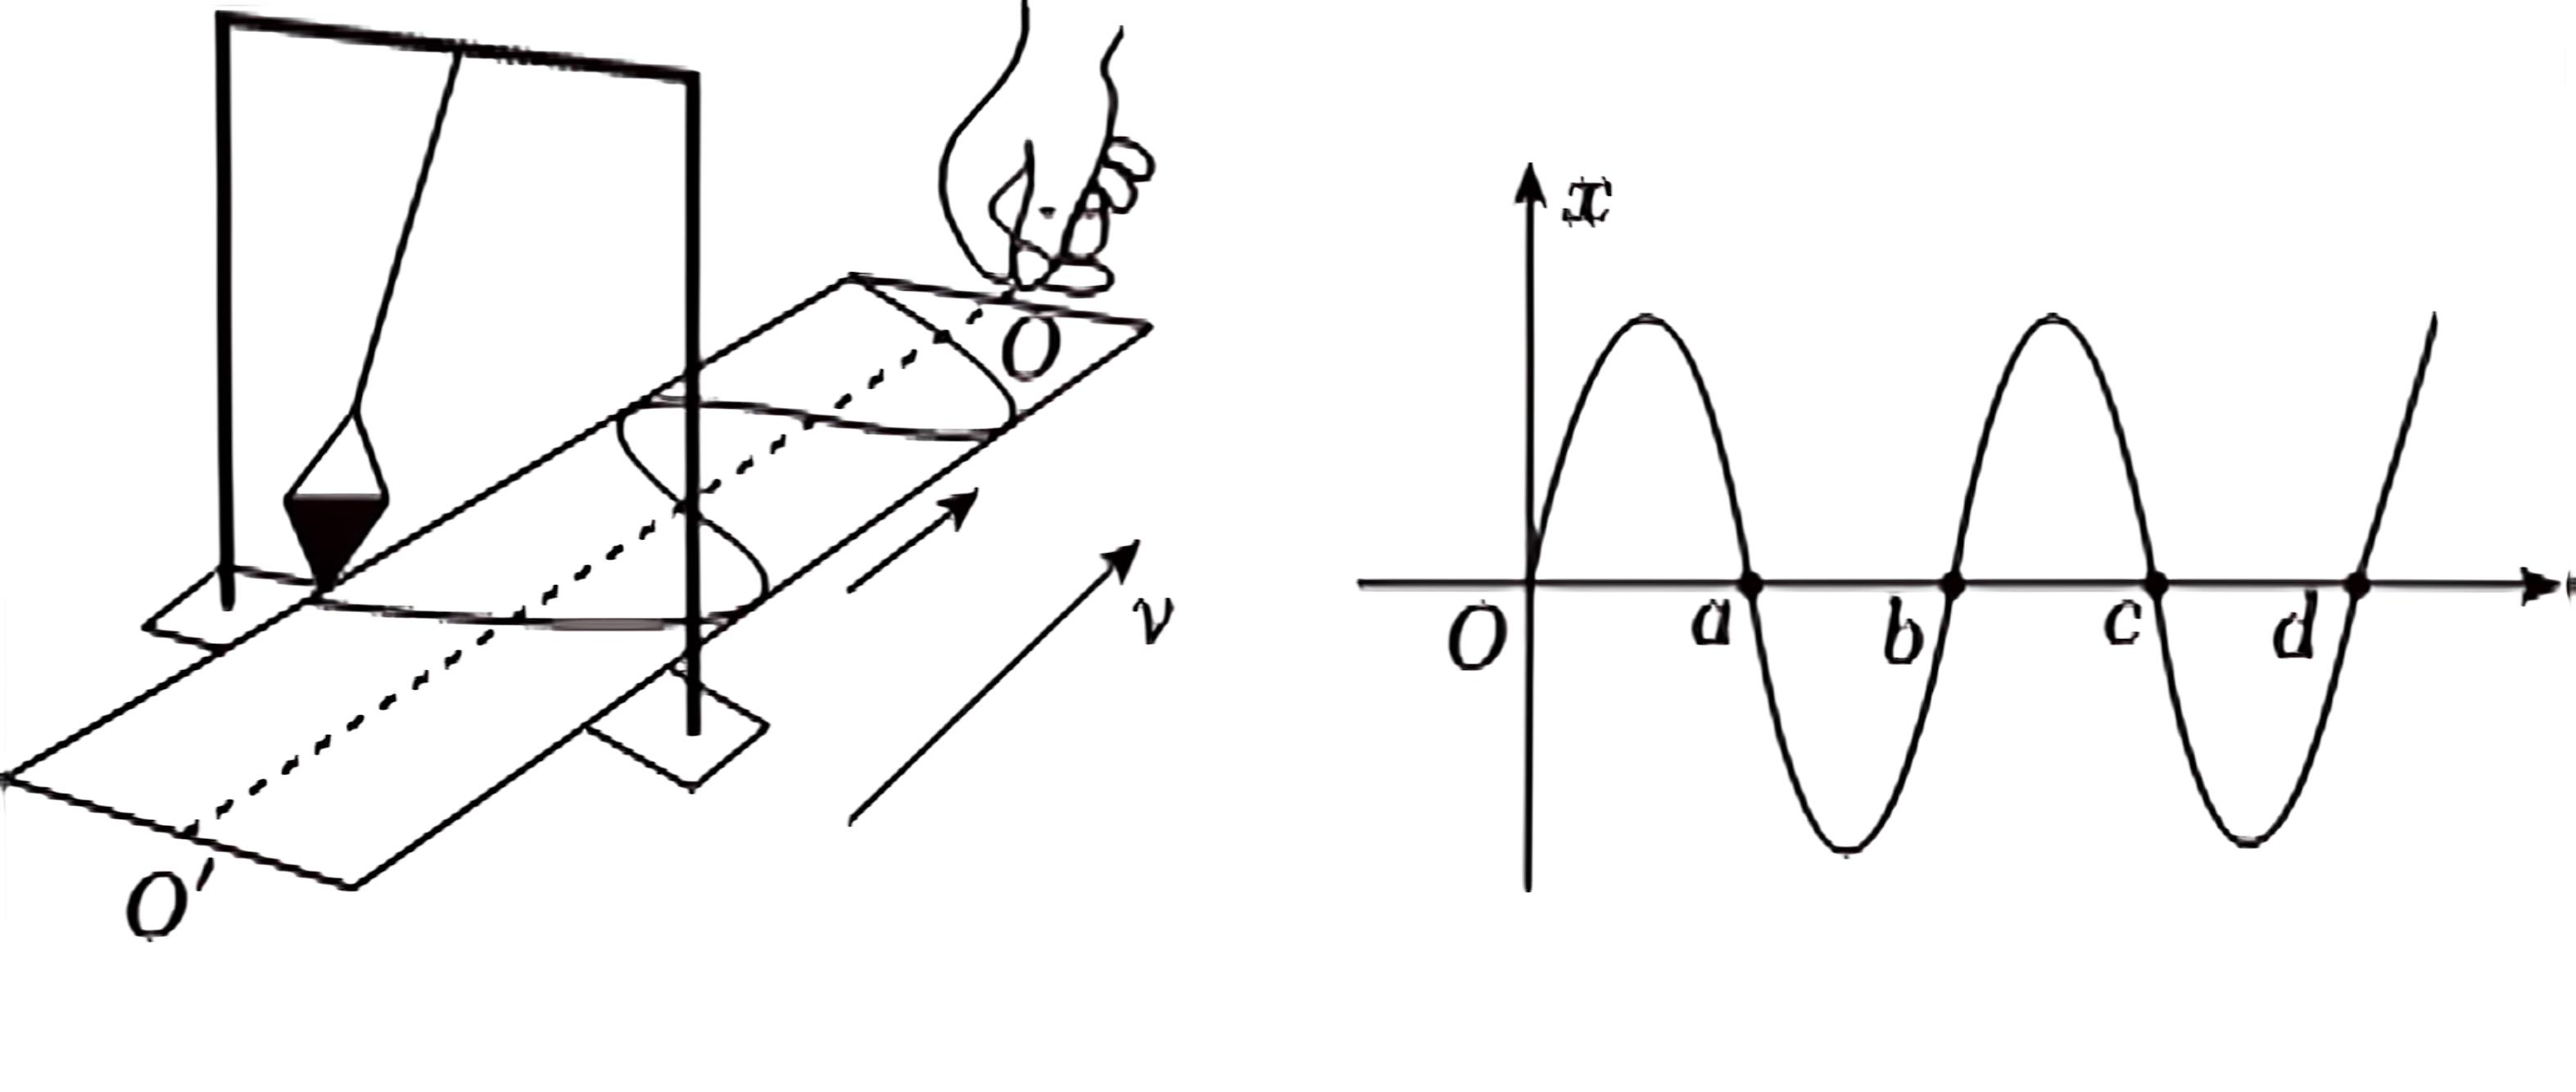
\includegraphics[width=0.6\textwidth]{figures/沙摆}
    \caption{沙摆实验示意图}
    \label{fig:sand_pendulum}
\end{figure}

本项目的AI辅助阻尼振动分析系统克服了上述缺点,为阻尼振动教学提供了全新解决方案:

\begin{enumerate}[leftmargin=*]
    \item 高精度轨迹追踪:系统可连续记录摆球位置,生成完整的位移-时间数据集,实现阻尼振动过程的精确量化;
    
    \item 多维度数据可视化:自动生成位置-时间曲线、速度-时间曲线、相位图和振幅衰减曲线,多角度展示阻尼振动特性;
    
    \item 参数自动计算:系统自动提取阻尼系数、固有频率、品质因数等关键参数,实现阻尼振动的定量分析;
    
    \item 交互式教学展示:通过软件界面可放大、缩小、暂停特定时间点的观察,或对比不同参数条件下的振动特性,增强教学交互性;
    
    \item 实验数据保存与共享:测量结果可导出为标准数据格式,便于学生课后分析或教师示范展示。
\end{enumerate}

在这些实验教学中,本团队探索将YOLO作为辅助教学工具,应用于单摆实验中。基于YOLO目标检测算法的教学软件能够实时、精准地捕捉摆球的位置信息,并自动生成运动数据文件。这些数据不仅为学生提供了更精确的实验数据,还帮助他们更直观地理解单摆的运动规律。学生可以利用这些数据通过软件绘制单摆的简谐运动图像、计算重力加速度和阻尼系数,这一创新使得学生能够更深入地理解阻尼运动的定量规律,将抽象的物理概念具象化,降低了实验操作难度,提高了实验的趣味性和教学效果。